%_____________________________________________________________________________________________ 
% LATEX Template: Department of Comp/IT BTech Project Reports
% Sample Chapter
% Sun Mar 27 10:25:35 IST 2011
%
% Note: Itemization, enumeration and other things not shown. A sample table is included.
%_____________________________________________________________________________________________ 

\chapter{Results}

\section{Evaluation Metrics}

\subsection{Precision}
Precision is the probability that a (randomly selected) retrieved document is relevant.
\begin{equation}
P = \frac{T_p}{T_p + F_p} \nonumber
\end{equation}

\subsection{Recall}
Recall is the probability that a (randomly selected) relevant document is retrieved in a search.
\begin{equation}
R = \frac{T_p}{T_p + F_n} \nonumber
\end{equation}

\subsection{Precision \& Recall}
The following graph illustrates the precision and recall of the prediction algorithm.
	\begin{figure}[t]
		\begin{center}
			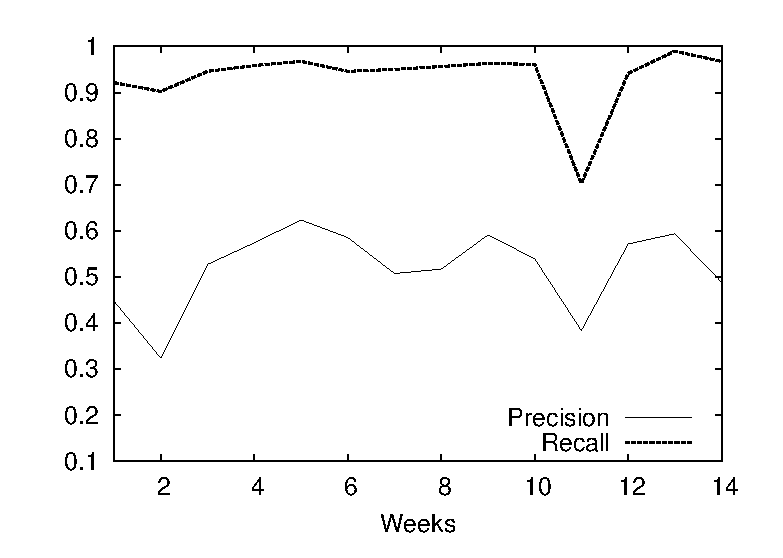
\includegraphics[width=10cm,height=8cm]{figures/precision.eps} 
			\caption{\small \sl Precision and Recall at 0.4 confidence.\label{fig:Label7}} 
		\end{center} 
	\end{figure}

\pagebreak

\subsection{Comparison between Failure Prediction at Various Confidence Values}
\begin{figure}[h]
		\begin{center}
			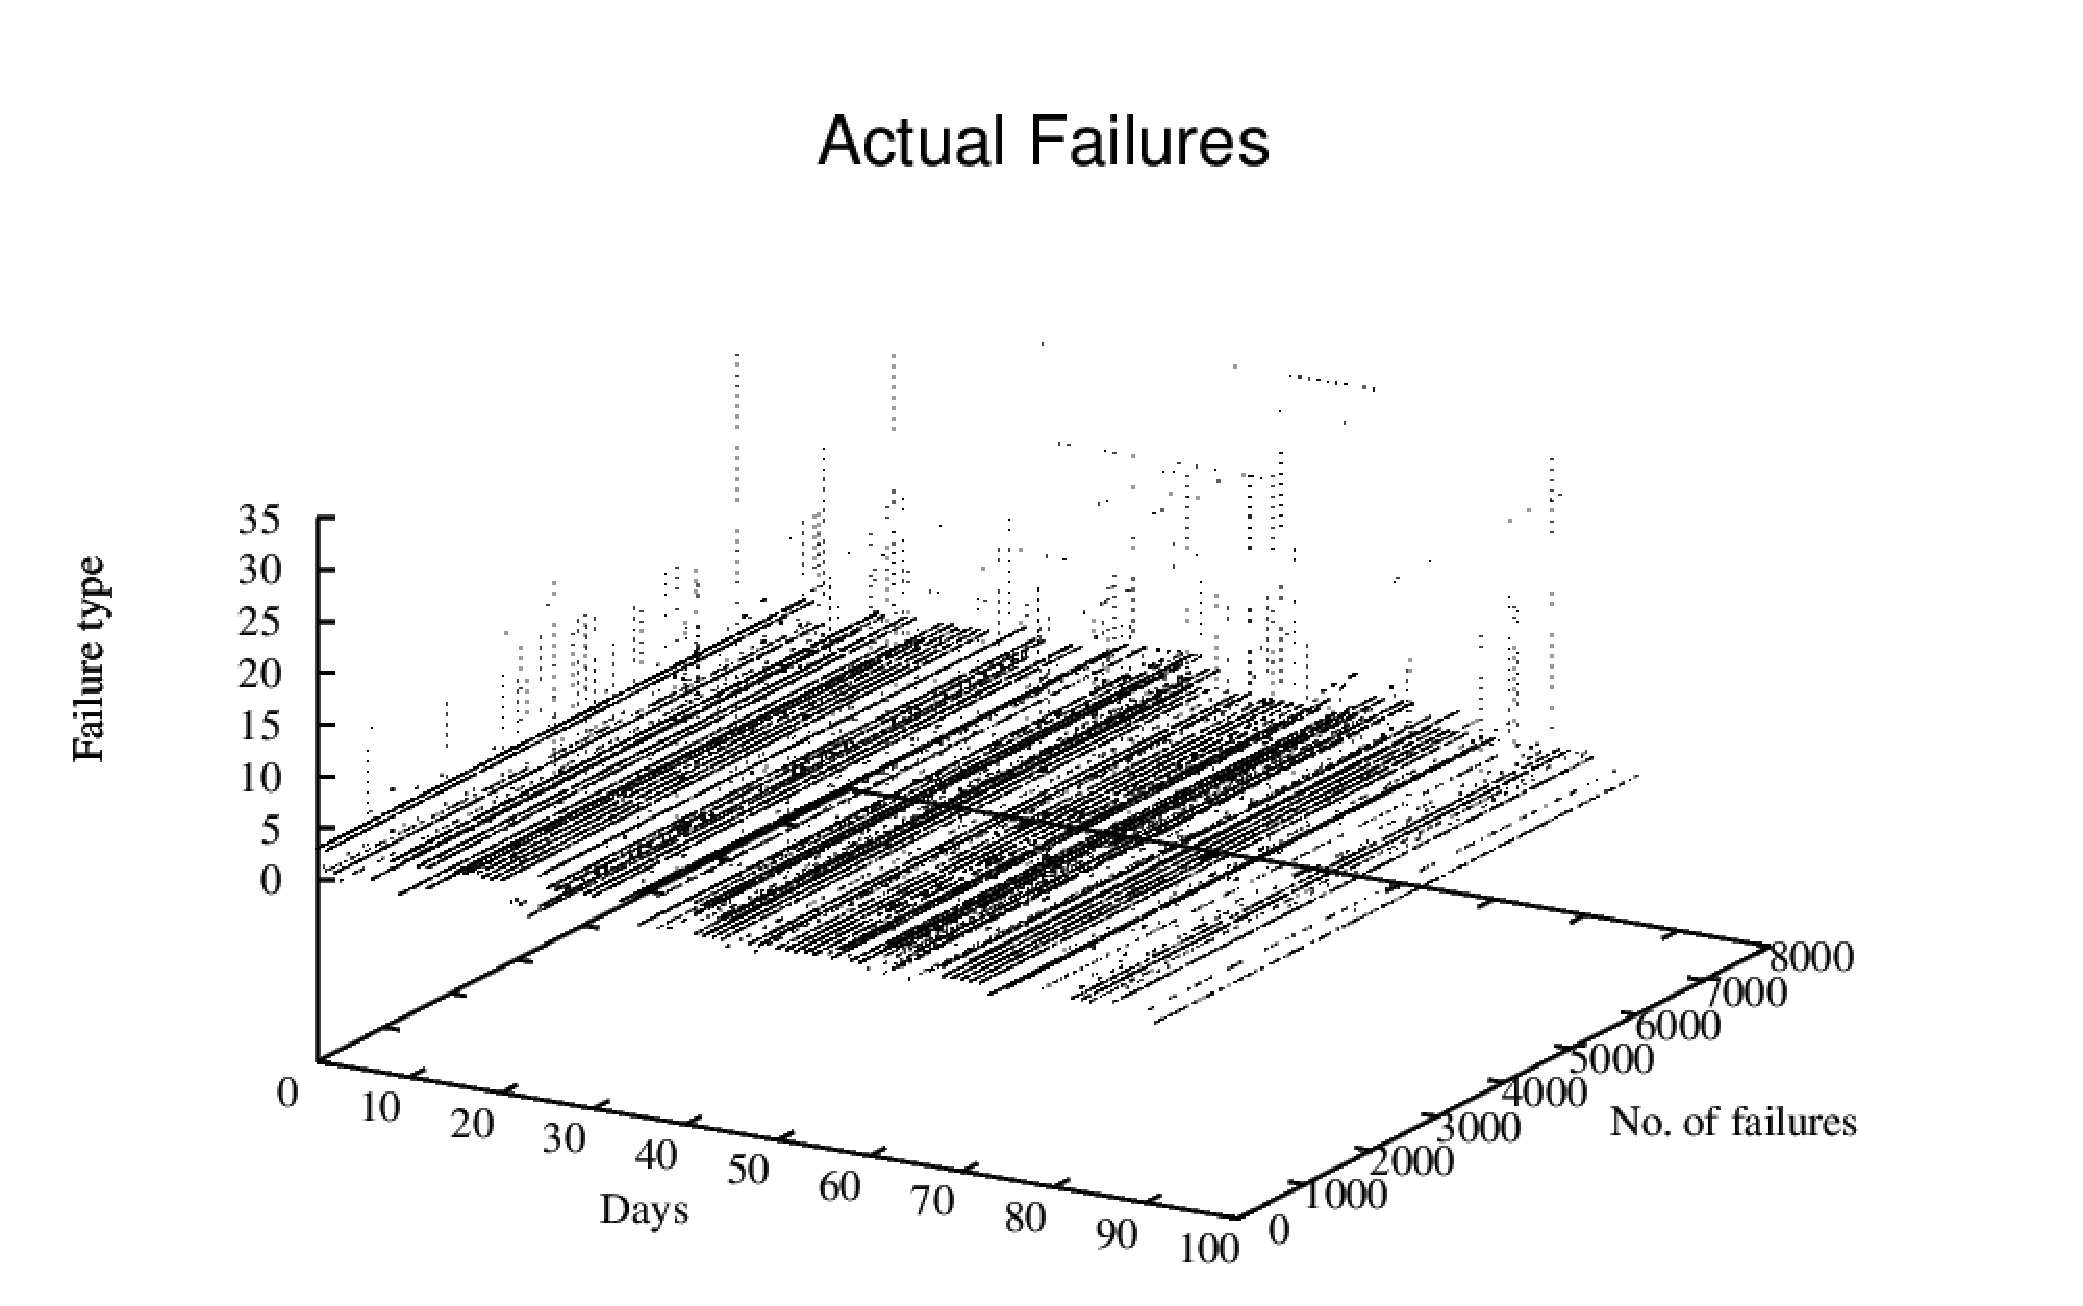
\includegraphics[width=15cm,height=10cm]{figures/actualfailures.eps} 
			\caption{\small \sl Actual Failures Plot\label{fig:Label7}} 
		\end{center} 
	\end{figure}

\newpage

\begin{figure}[h]
		\begin{center}
			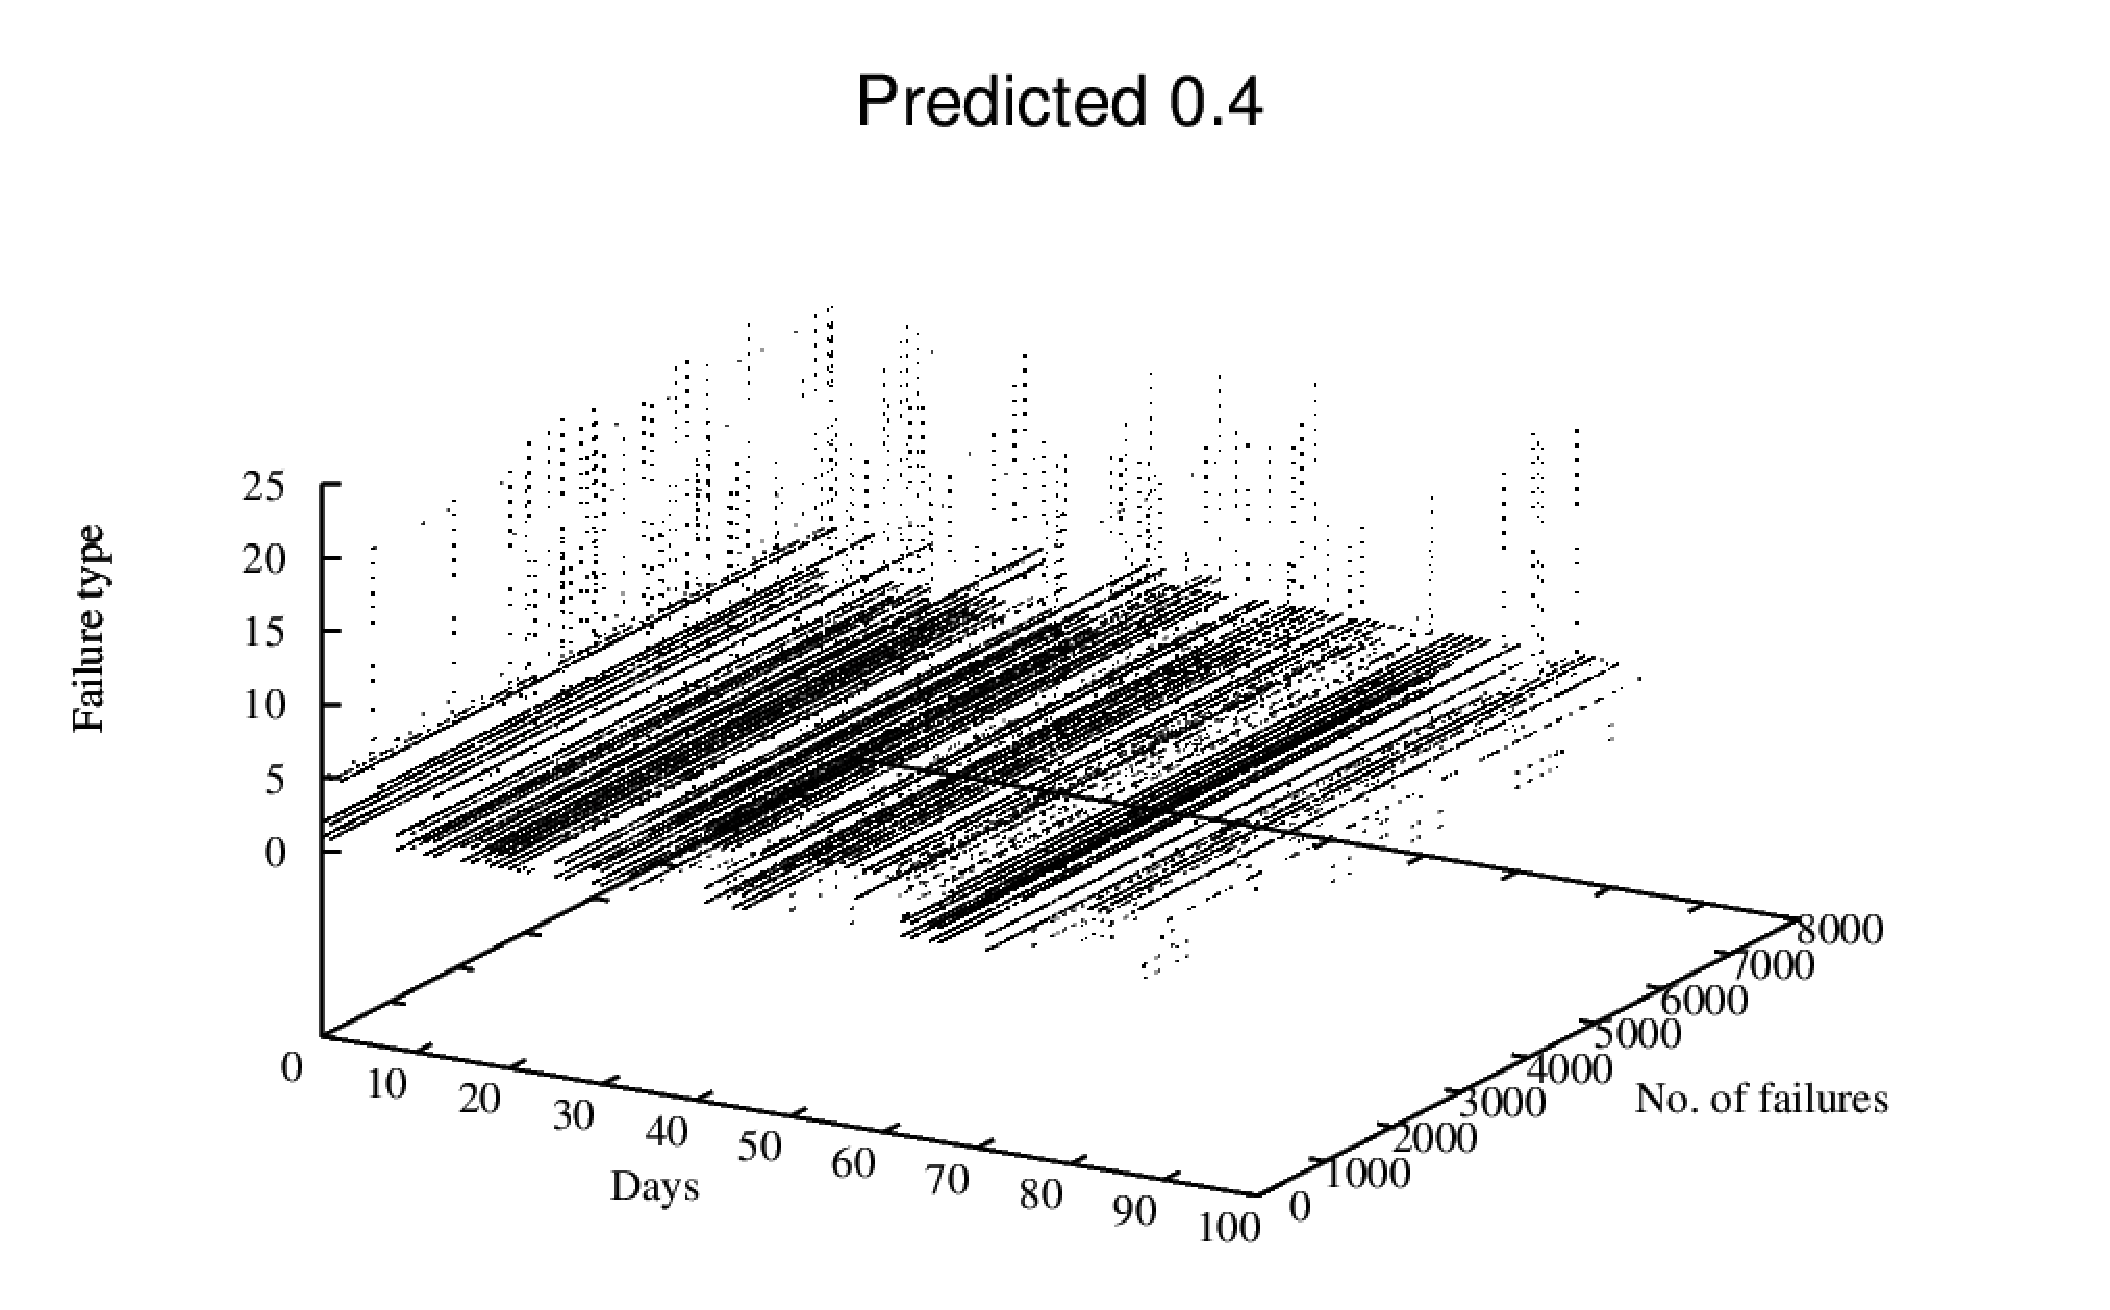
\includegraphics[width=15cm,height=10cm]{figures/predicted0.4.eps} 
			\caption{\small \sl Predicted Failures at 0.4 Confidence\label{fig:Label7}} 
		\end{center} 
	\end{figure}

\newpage

\begin{figure}[h]
		\begin{center}
			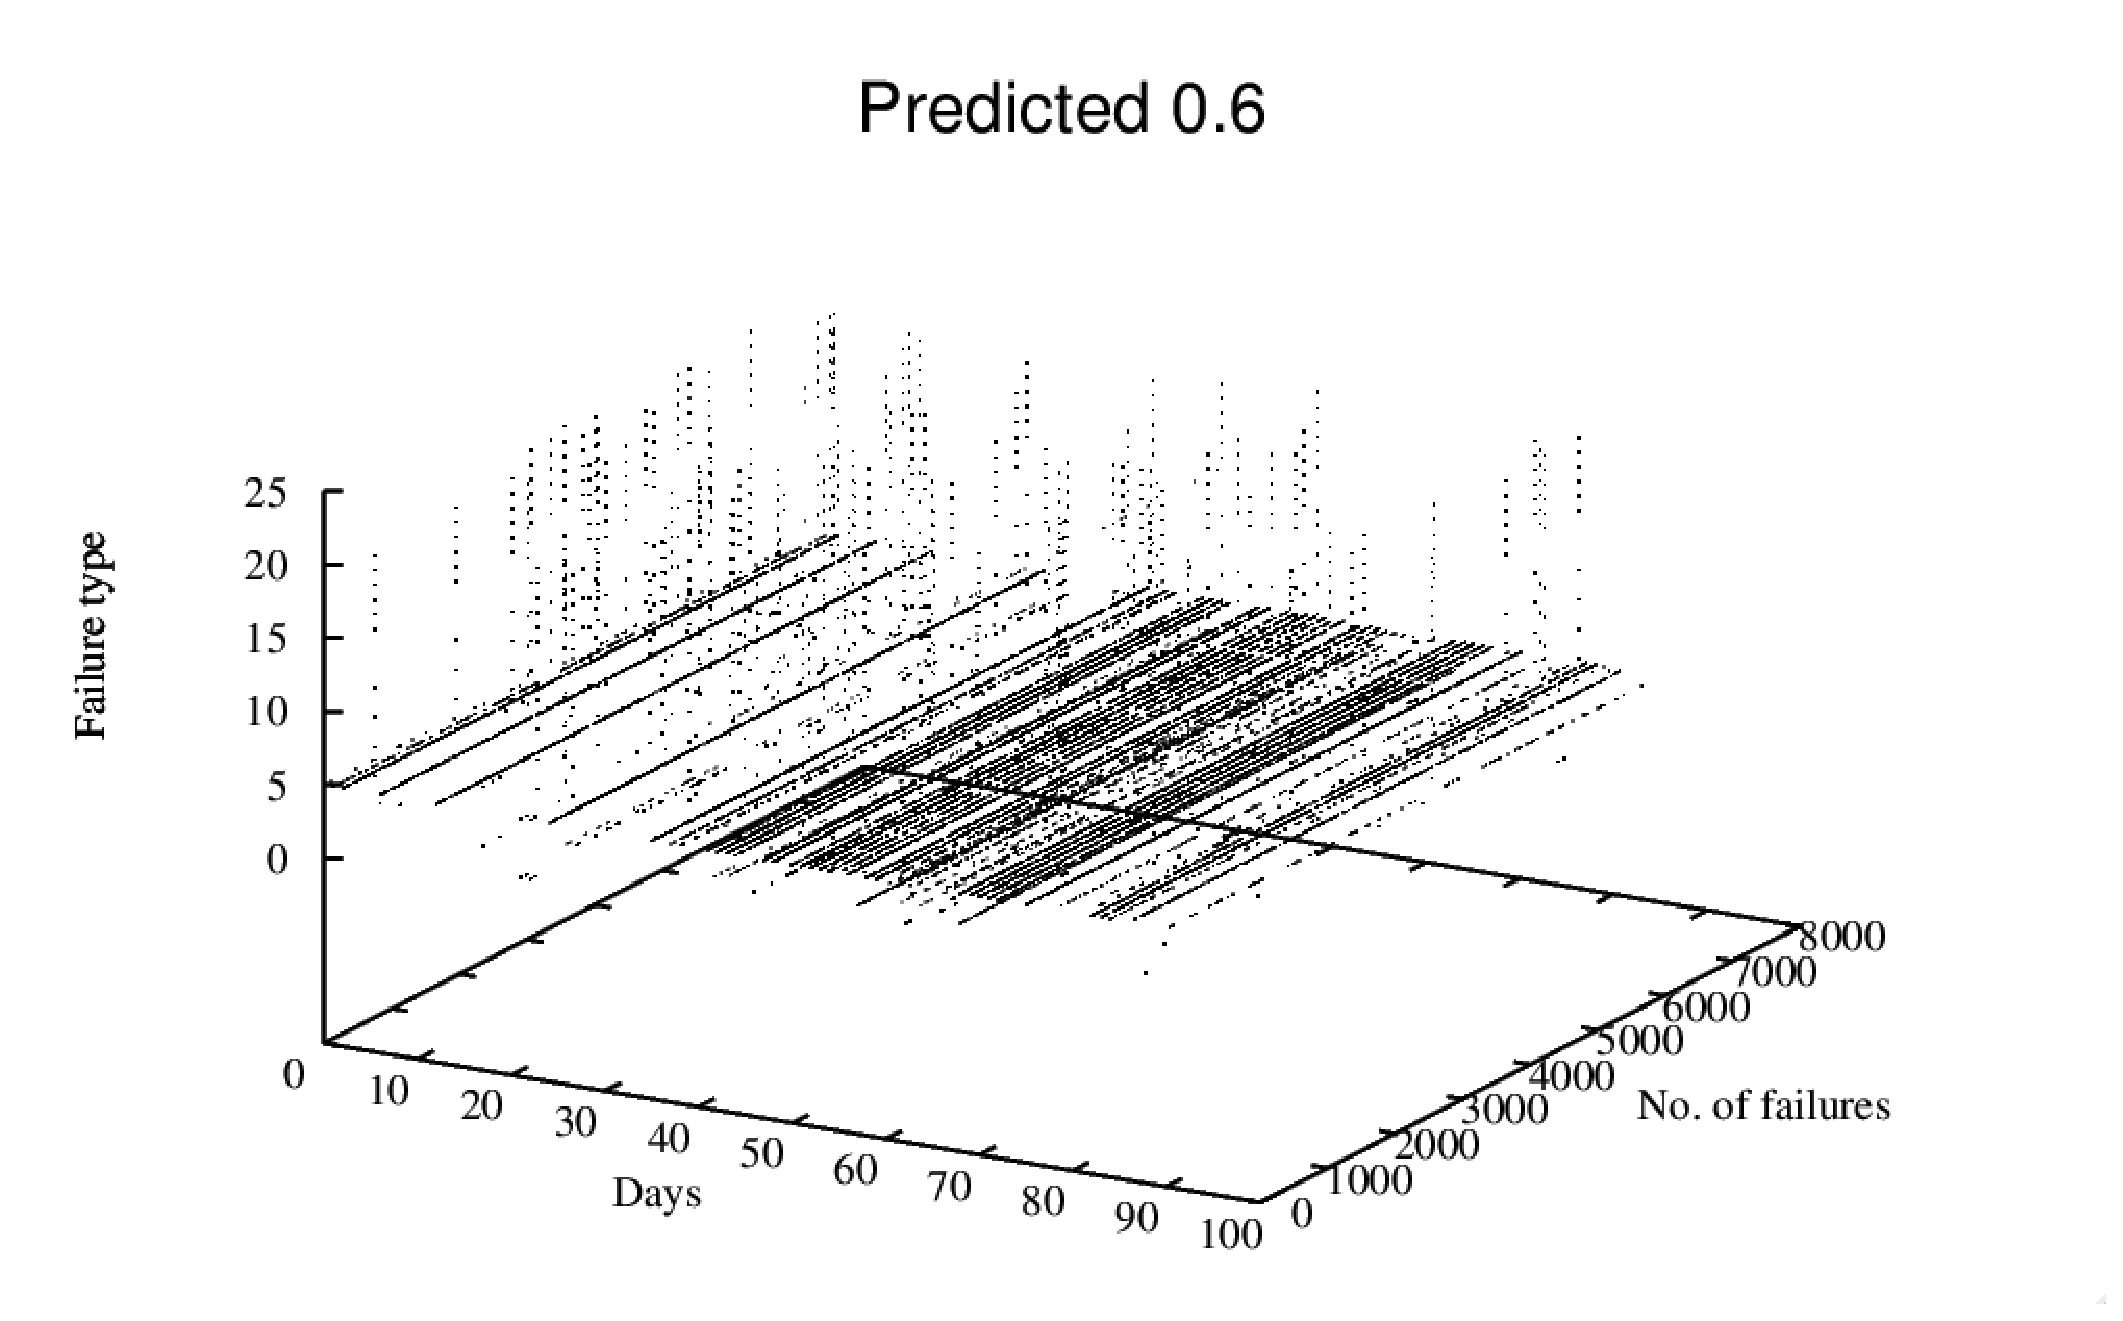
\includegraphics[width=15cm,height=10cm]{figures/predicted0.6.eps} 
			\caption{\small \sl Predicted Failures at 0.6 Confidence\label{fig:Label7}} 
		\end{center} 
	\end{figure}


%Scatter 3D plot (3 graps -> actual, predicted for 0.4 and predicted for 0.6)

%_____________________________________________________________________________________________ 
